
    \centering
 
    \tikzsetnextfilename{ej_esfera_elemental} 
    
    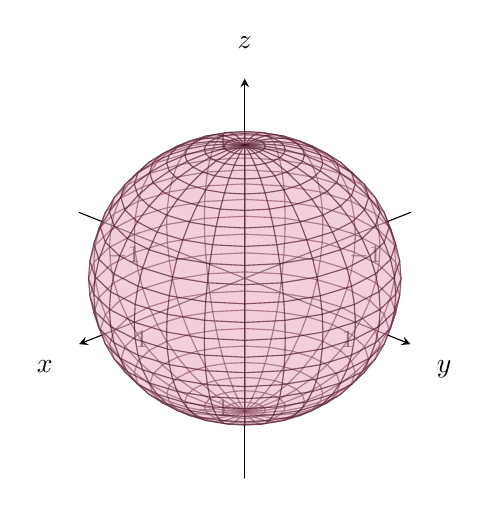
\begin{tikzpicture}[line cap=round, line join=round]
        \begin{axis}[
            view={135}{25}, % Cámara clásica
            width=10cm,
            height=10cm,
            axis lines=center,
            % Ajustamos los ejes a la esfera de radio 1
            xmin=-1.5, xmax=1.5, 
            ymin=-1.5, ymax=1.5,
            zmin=-1.5, zmax=1.5,
            xlabel={$x$},
            ylabel={$y$},
            zlabel={$z$},
            % Anclaje perfecto de letras
            every axis x label/.style={at={(ticklabel* cs:1.05)},anchor=north east},
            every axis y label/.style={at={(ticklabel* cs:1.05)},anchor=north west},
            every axis z label/.style={at={(ticklabel* cs:1.05)},anchor=south},
            ticklabel style={font=\small},
        ]

        % Esfera unitaria x^2 + y^2 + z^2 = 1 (Roja transparente)
        \addplot3[
            surf,
            opacity=0.4,
            color=purple!30,
            faceted color=purple!30!black,
            samples=25, % Reducido para no saturar la memoria
            domain=0:360,
            y domain=0:180,
            z buffer=sort
        ]
        ({cos(x)*sin(y)}, {sin(x)*sin(y)}, {cos(y)});

        \end{axis}
    \end{tikzpicture}
    \caption{Representación de la región $W$.}

